

%% This file was auto-generated by IPython.
%% Conversion from the original notebook file:
%%
\documentclass[11pt,english]{article}

%% This is the automatic preamble used by IPython.  Note that it does *not*
%% include a documentclass declaration, that is added at runtime to the overall
%% document.

\usepackage{amsmath}
\usepackage{amssymb}
\usepackage{graphicx}
\usepackage{grffile}
\usepackage{ucs}
\usepackage[utf8x]{inputenc}

% Scale down larger images
\usepackage[export]{adjustbox}

%fancy verbatim
\usepackage{fancyvrb}
% needed for markdown enumerations to work
\usepackage{enumerate}

% Slightly bigger margins than the latex defaults
\usepackage{geometry}
\geometry{verbose,tmargin=3cm,bmargin=3cm,lmargin=2.5cm,rmargin=2.5cm}

% Define a few colors for use in code, links and cell shading
\usepackage{color}
\definecolor{orange}{cmyk}{0,0.4,0.8,0.2}
\definecolor{darkorange}{rgb}{.71,0.21,0.01}
\definecolor{darkgreen}{rgb}{.12,.54,.11}
\definecolor{myteal}{rgb}{.26, .44, .56}
\definecolor{gray}{gray}{0.45}
\definecolor{lightgray}{gray}{.95}
\definecolor{mediumgray}{gray}{.8}
\definecolor{inputbackground}{rgb}{.95, .95, .85}
\definecolor{outputbackground}{rgb}{.95, .95, .95}
\definecolor{traceback}{rgb}{1, .95, .95}

% new ansi colors
\definecolor{brown}{rgb}{0.54,0.27,0.07}
\definecolor{purple}{rgb}{0.5,0.0,0.5}
\definecolor{darkgray}{gray}{0.25}
\definecolor{lightred}{rgb}{1.0,0.39,0.28}
\definecolor{lightgreen}{rgb}{0.48,0.99,0.0}
\definecolor{lightblue}{rgb}{0.53,0.81,0.92}
\definecolor{lightpurple}{rgb}{0.87,0.63,0.87}
\definecolor{lightcyan}{rgb}{0.5,1.0,0.83}

% Framed environments for code cells (inputs, outputs, errors, ...).  The
% various uses of \unskip (or not) at the end were fine-tuned by hand, so don't
% randomly change them unless you're sure of the effect it will have.
\usepackage{framed}

% remove extraneous vertical space in boxes
\setlength\fboxsep{0pt}

% codecell is the whole input+output set of blocks that a Code cell can
% generate.

% TODO: unfortunately, it seems that using a framed codecell environment breaks
% the ability of the frames inside of it to be broken across pages.  This
% causes at least the problem of having lots of empty space at the bottom of
% pages as new frames are moved to the next page, and if a single frame is too
% long to fit on a page, will completely stop latex from compiling the
% document.  So unless we figure out a solution to this, we'll have to instead
% leave the codecell env. as empty.  I'm keeping the original codecell
% definition here (a thin vertical bar) for reference, in case we find a
% solution to the page break issue.

%% \newenvironment{codecell}{%
%%     \def\FrameCommand{\color{mediumgray} \vrule width 1pt \hspace{5pt}}%
%%    \MakeFramed{\vspace{-0.5em}}}
%%  {\unskip\endMakeFramed}

% For now, make this a no-op...
\newenvironment{codecell}{}

 \newenvironment{codeinput}{%
   \def\FrameCommand{\colorbox{inputbackground}}%
   \MakeFramed{\advance\hsize-\width \FrameRestore}}
 {\unskip\endMakeFramed}

\newenvironment{codeoutput}{%
   \def\FrameCommand{\colorbox{outputbackground}}%
   \vspace{-1.4em}
   \MakeFramed{\advance\hsize-\width \FrameRestore}}
 {\unskip\medskip\endMakeFramed}

\newenvironment{traceback}{%
   \def\FrameCommand{\colorbox{traceback}}%
   \MakeFramed{\advance\hsize-\width \FrameRestore}}
 {\endMakeFramed}

% Use and configure listings package for nicely formatted code
\usepackage{listingsutf8}
\lstset{
  language=python,
  inputencoding=utf8x,
  extendedchars=\true,
  aboveskip=\smallskipamount,
  belowskip=\smallskipamount,
  xleftmargin=2mm,
  breaklines=true,
  basicstyle=\small \ttfamily,
  showstringspaces=false,
  keywordstyle=\color{blue}\bfseries,
  commentstyle=\color{myteal},
  stringstyle=\color{darkgreen},
  identifierstyle=\color{darkorange},
  columns=fullflexible,  % tighter character kerning, like verb
}

% The hyperref package gives us a pdf with properly built
% internal navigation ('pdf bookmarks' for the table of contents,
% internal cross-reference links, web links for URLs, etc.)
\usepackage{hyperref}
\hypersetup{
  breaklinks=true,  % so long urls are correctly broken across lines
  colorlinks=true,
  urlcolor=blue,
  linkcolor=darkorange,
  citecolor=darkgreen,
  }

% hardcode size of all verbatim environments to be a bit smaller
\makeatletter 
\g@addto@macro\@verbatim\small\topsep=0.5em\partopsep=0pt
\makeatother 

% Prevent overflowing lines due to urls and other hard-to-break entities.
\sloppy




\begin{document}



\begin{codecell}


\begin{codeinput}
\begin{lstlisting}
#read in file - no utf8
lines = [line.strip() for line in open('100_biggest_cities_germany.txt')]
lines = [line.split("\t") for line in lines]

cities = []

#create dict
for line in lines[1:]:
    cities.append(dict(zip(lines[0], line)))

#type casting
for city in cities:
    city['Lat'] = (float) (city['Lat'])
    city['Long'] = (float) (city['Long'])
    city['Population'] = (int) (city['Population'])

print len(cities)
\end{lstlisting}
\end{codeinput}
\begin{codeoutput}


\begin{Verbatim}[commandchars=\\\{\}]
100
\end{Verbatim}

\end{codeoutput}

\end{codecell}

\begin{codecell}


\begin{codeinput}
\begin{lstlisting}
lats = [x['Lat'] for x in cities]
longs = [x['Long'] for x in cities]
pops = [x['Population'] for x in cities]


min_lat = min(lats)
max_lat = max(lats)
mean_lat = sum(lats)/len(lats)

min_long = min(longs)
max_long = max(longs)
mean_long = sum(longs)/len(longs)

min_pop = min(pops)
max_pop = max(pops)
mean_pop = sum(pops)/len(pops)

\end{lstlisting}
\end{codeinput}

\end{codecell}

\begin{codecell}


\begin{codeinput}
\begin{lstlisting}
#helper functions
from math import cos, asin, sqrt

def points_on_circle(xpos, ypos, radius, n):
    points = []
    y_tmp = []
    
    xs = [x  for x in linspace(0, radius*2, n, endpoint = False)]
    
    for x in xs:
        x = x - radius
        y = cos(asin( x / radius ))
        x = x + xpos
        y_tmp.append((x, y))
        
    #circular output
    for (x, y) in y_tmp[::2]:
        points.append((x, ypos+y))
        
    for (x, y) in [p for p in reversed(y_tmp)][::2]:
        points.append((x, ypos-y))
        
    return points

def winner(goal, cities):
    d = [sqrt(abs(c[0]-goal[0])*abs(c[1]-goal[1])) for c in cities]
    return d.index(min(d))

\end{lstlisting}
\end{codeinput}

\end{codecell}

\begin{codecell}


\begin{codeinput}
\begin{lstlisting}
from math import log
from numpy import linspace, array, random
import matplotlib.pyplot as plt


#SETUP
iterations = 2000
neurons = 300
input_dim = 2

lro = 0.3
so  = 150

T1 = iterations/log(so)

circle = points_on_circle(mean_long, mean_lat, 4, neurons)
circle = array(circle)

#random weights
#ws = random.rand(neurons, input_dim)

#lets roll with not so random weights
ws = circle
cities = [(city['Long'], city['Lat']) for city in cities]
cities = array(cities)

plt.scatter([c[0] for c in circle], [c[1] for c in circle])

\end{lstlisting}
\end{codeinput}
\begin{codeoutput}




\begin{verbatim}
<matplotlib.collections.PathCollection at 0x340abd0>
\end{verbatim}



\begin{center}
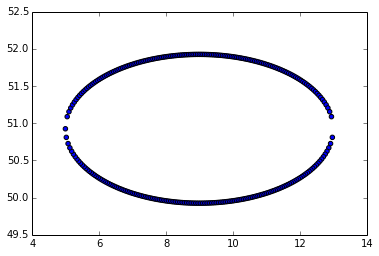
\includegraphics[max size={0.7\textwidth}{0.9\textheight}]{NN_ChristopheQuignon_011214_files/NN_ChristopheQuignon_011214_3_1.png}
\par
\end{center}

\end{codeoutput}

\end{codecell}

\begin{codecell}


\begin{codeinput}
\begin{lstlisting}
#TSP
from numpy import exp, where
from random import shuffle

plt.ion()

#for n iterations
for n in range(iterations):
    
    #Value update
    sigma = so*exp(-n/T1)
    learning_rate = lro * exp(-n/iterations)
    neighbors = sigma * exp(-n/iterations)
    
    #shuffle(cities)
    

    for city in cities:
        #find closest between weights and activation
        winner_index = winner(city, ws)
        
        #update winning neuron
        x = city
        wi = ws[winner_index]
        ws[winner_index] = wi + (learning_rate*(x[0]-wi[0]), learning_rate*(x[1]-wi[1]))
        
        #cooperation
        for d in range(1, int( neighbors/2)):
            i_up = (winner_index+d)%len(circle)
            i_down = (winner_index-d)%len(circle)
            
            lr = learning_rate * exp(-((d ** 2)/(2*sigma**2) ))
            
            ws[i_up] = ws[i_up] + (lr*(x[0]-ws[i_up][0]), lr*(x[1]-ws[i_up][1]))
            ws[i_down] = ws[i_up] + (lr*(x[0]-ws[i_down][0]), lr*(x[1]-ws[i_down][1]))
            
            
    #drawing is expensive
    if ((n%400) ==0):
    #print n
        
        print 'neighbors = ', neighbors
        
        plt.clf()
        plt.axes().set_aspect(1.5)
        
        plt.scatter ([c[0] for c in cities], [c[1] for c in cities], c='y', s = 40)
        
        last_w = ws[-1]
        for w in ws:
            plt.scatter(w[0], w[1])
            plt.plot([last_w[0], w[0]], [last_w[1], w[1]], c = 'b')
            last_w = w
        plt.draw()
        show()

\end{lstlisting}
\end{codeinput}
\begin{codeoutput}


\begin{Verbatim}[commandchars=\\\{\}]
neighbors =  150.0
\end{Verbatim}

\begin{center}
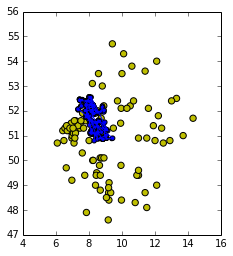
\includegraphics[max size={0.7\textwidth}{0.9\textheight}]{NN_ChristopheQuignon_011214_files/NN_ChristopheQuignon_011214_4_1.png}
\par
\end{center}

\begin{Verbatim}[commandchars=\\\{\}]
neighbors =  20.2571584599
\end{Verbatim}

\begin{center}
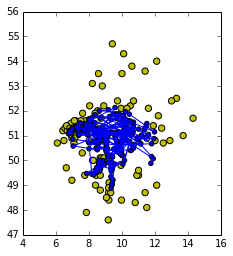
\includegraphics[max size={0.7\textwidth}{0.9\textheight}]{NN_ChristopheQuignon_011214_files/NN_ChristopheQuignon_011214_4_3.png}
\par
\end{center}

\begin{Verbatim}[commandchars=\\\{\}]
neighbors =  7.43635772927
\end{Verbatim}

\begin{center}
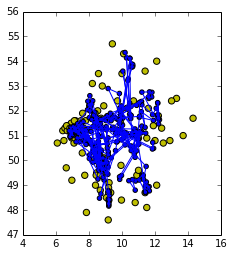
\includegraphics[max size={0.7\textwidth}{0.9\textheight}]{NN_ChristopheQuignon_011214_files/NN_ChristopheQuignon_011214_4_5.png}
\par
\end{center}

\begin{Verbatim}[commandchars=\\\{\}]
neighbors =  2.72987035112
\end{Verbatim}

\begin{center}
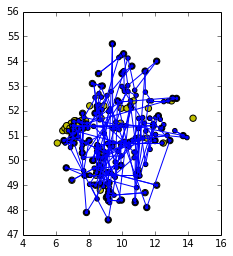
\includegraphics[max size={0.7\textwidth}{0.9\textheight}]{NN_ChristopheQuignon_011214_files/NN_ChristopheQuignon_011214_4_7.png}
\par
\end{center}

\begin{Verbatim}[commandchars=\\\{\}]
neighbors =  1.00212932261
\end{Verbatim}

\begin{center}
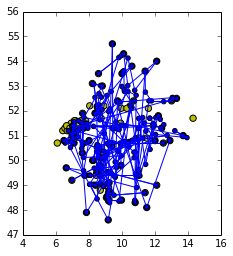
\includegraphics[max size={0.7\textwidth}{0.9\textheight}]{NN_ChristopheQuignon_011214_files/NN_ChristopheQuignon_011214_4_9.png}
\par
\end{center}

\end{codeoutput}

\end{codecell}

\begin{codecell}


\begin{codeinput}
\begin{lstlisting}
#Conclusion:
#the SOM sometimes has a good intermediate plan
#but fails to crystalize at the right time.
\end{lstlisting}
\end{codeinput}

\end{codecell}



\end{document}

